\documentclass[implementacija.tex]{subfiles}
\usepackage{subfiles}
\documentclass[12pt,oneside]{memoir} 
\usepackage[latinica]{matfmaster} 

\begin{document}
K\^{o}d svake Android aplikacije se nalazi u direktorijumu: \textbf{app}. Osnovnu strukturu \textbf{app} direktorijuma bilo koje Android aplikacije čine poddirektorijumi: 

\begin{itemize}
\item \textit{build} sa izvršnom verzijom koda i svim generisanim datotekama,
\item \textit{libs} sa eksternim bibliotekama odnosno bibliotekama koje nisu deo Androida i programskih jezika Java ili Kotlin i
\item \textit{src} sa izvornim kodom.
\end{itemize}

 Direktorijum \textbf{src} se uglavnom sastoji od sledećih poddiretkorijuma: 
\begin{itemize}
\item \textit{AndroidTest} u kom se smeštaju svi testovi koje je potrebno pokrenuti na Android uređaju, 
\item \textit{test} u kom se smeštaju svi testovi za testiranje jedinica koda (eng. \textit{unit tests})
\item \textit{main} u kom se nalazi ceo izvorni k\^{o}d.
\end{itemize}

Projekat implementacije upravljača za digitalnu televiziju je smešten u direktorijumu pod nazivom \textit{RemoteControlApp}. Srž aplikacije se nalazi u \textbf{main} poddirektorijumu, a za ovu aplikaciju ovaj direktorijum ima sledeću strukturu:
\begin{itemize}
\item \textit{AndroidMainifest.xml} --- datoteka koji opisuje glavne postavke aplikacije,
\item \textit{res} --- direktorijum sa svim XML datotekama koje čine korisnički interfejs (eng. \textit{user interface}) aplikacije,
\item \textit{java} --- direktorijum sa svim klasama i interfejsima aplikacije
\item \textit{proto} --- direktorijum sa \textit{.proto} datotekama koje su neophodne za korišćenje \textit{Google Cloud API}-ja.
\end{itemize}

\section{Upravljanje procesom izgradnje i određivanje zavisnosti aplikacije}

Važne datoteke pri postavljanju projekta su \textbf{\textit{build.gradle}} datoteke koje služe da  upravljaju procesom izgradnje i odrede zavisnosti (eng. \textit{dependency}) aplikacije. Ove datoteke se generišu automatski pri kreiranju projekta, ali je moguće dodati sve dodatne zavisnosti koje budu potrebne. Postoje dva tipa ovih datoteka --- na nivou projekta i na nivou modula. Datoteku na nivou projekta čini skup pravila koji važi za ceo projekat, dok datoteke na nivou modula čine pravila za modul u kom se nalazi datoteka. Svaka ova datoteka se sastoji od vise blokova koji grupišu unutar sebe pravila, odnosno opcije koje se primenjuju.

Za uspešno korišćenje \textit{Google Cloud} servisa u aplikaciji, neophodno je uvesti podršku za obradu \textit{Protobuf} (skraćeno od eng. \textit{Protocol Buffers}) datoteka. \textit{Protobuf} je interfejs za definiciju jezika (eng. \textit{Interface Definition Language}, skraćeno IDL) koji definiše strukturu podataka i programski interfejs. \cite{sajt:protobuf} Omogućava usaglašeost pri deljenju struktuiranih podataka između različitih sistemskih platformi i jezika programiranja. Neophodno je unutar bloka \textit{plugins} dodati dodatak \verb|id 'com.google.protobuf'| kako bi se obezbedila adekvatna podrška. Takođe u okviru bloka \textit{protobuf}, se dodaju opcije za korišćenje protobuf-a. Tačne zavisnosti koje je potrebno dodati biće navedene kod opisa implementacije glasovnih komandi gde će biti i objašnjena povezanost \textit{Google cloud} servisa i \textit{protobuf}-a.

\section{Potrebne dozvole i informacije za pokretanje aplikacije}

Informacije potrebne za pokretanje i instalaciju aplikacije čine datoteku \textit{AndroidManifest.xml}. U ovoj datoteci su definisane sve dozvole koje aplikacija zahteva od uređaja sa kog se pokreće aplikacija: pristup internetu, stanju bežične mreže (eng. \textit{WiFi}), stanju telefona, vibracija i  snimanje audio sadržaja. Pregled ovih dozvola je dat u listingu \ref{lst:manifestApp}. Kao što je navedeno u delu \ref{sec:manifest} glavna etiketa koja mora postojati je za aplikaciju i u okviru nje su postavljene vrednosti naziva aplikacije, slika kojom je aplikacija predstavljena, ciljani API nivo kao i dve aktivnosti koje se pojavljuju. Prva aktivnost je \textit{ChooseConnection}, koja je odabir uređaja sa kojim će se korisnik povezati i ona je obeležena kao glavna aktivnost. Druga aktivnost je \textit{RemoteView} koja čini prikaz daljinskog upravljača. 

\lstinputlisting[language=XML, caption= {Odobrenja definisana u datoteci \textit{AndroidManifest.xml}}, label={lst:manifestApp}]{implementacije/kodovi/AppManifest.xml}


\section{Resursi aplikacije}
Direktorijum u kom se smeštaju svi resursi aplikacije se naziva \textit{res}. Resursi koji se mogu čuvati su slike, planovi (eng. \textit{layout}), stringovi, stilovi itd. Moguće je čuvati iste resurse u različitim dimenzijama kako bi u zavisnosti od dimenzija i podešavanja uređaja bili odabrani odgovarajući resursi. Direktorijum \textit{drawable} skladišti slike. Za potrebe projekta formirane su i sačuvane slike za strelicu koja je predstavljena trouglom, ovalno dugme i dugme za prekid konekcije. 

Vrednosti, boje i dimenzije za različite resurse se skladište u direktorijumu \textit{values}. Datoteka \textit{colors.xml} sadrži boje korišćene za kreiranje interfejsa. Stringovi potrebni za dizajn korisničkog interfejsa su sačuvani u \textit{strings.xml}. Kolor shema, odnosno tema aplikacije je definisana u \textit{themes/themes.xml} odakle se može uočiti da boje koje se koriste za korisnički interfejs su nijanse plave boje. 

Svaki ekran sa kojim se korisnik može susresti mora imati korisnički interfejs koji ima svoj plan opisan unutar XML datoteke. Skup svih planova je smešten unutar direktorijuma \textit{layout} koji kod ove aplikacije ima sledeće XML datoteke:
\begin{description}
\item[\textbf{activity\_choose\_stb}] predstavlja plan ekrana za odabir konekcije, odnosno STB uređaja sa kojim korisnik želi da se poveže. Ovaj plan je inicijalno sastavljen od tri komponente koje se prikazuju po potrebi kada im se u kodu podesi vidljivost. Komponente su:
\begin{itemize}
    \item \textit{RecyclerView} sa id-jem \textit{@+id/rv\_boxes\_list} koji prikazuje spisak uređaja na mreži
    \item \textit{ProgressBar} koji može poslužiti prilikom učitavanja
    \item \textit{RelativeLayout} sa id-jem \textit{@+id/rl\_pairing\_container} koji se sastoji od tekstualnog polja sa uputstvom za unos koda za uparivanje, polja za unos koda i dugmeta za potvrdu 
\end{itemize}
\item[\textbf{remote\_control\_scene}] predstavlja izgled daljinskog upravljača. Korisnički interfejs ovog plana kao i shematski plan zajedno sa svim ograničenjima se može videti na slici \ref{fig:remoteScena}. Ovaj plan se sastoji od velikog broja dugmica koji su vizuelno intuitivni korisniku o svojim funkcionalnostima.
\item[\textbf{stb\_view}] predstavlja jedan element \textit{RecyclerView}. Sastoji se od polja za tekst koje predstavlja ime uređaja. 
\end{description}

%=================== SLIKA ======================================
\begin{figure}[!ht]
  \centering
  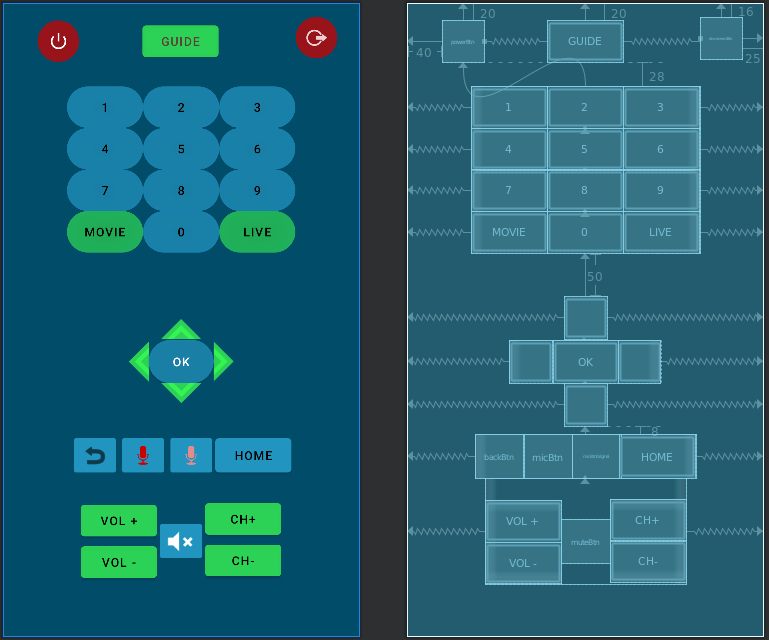
\includegraphics[width=\textwidth]{Implementacija/snimci_ekrana/remote_control_scene.png}
  \caption{Korisnički interfejs i shematski plan daljinskog upravljača}
  \label{fig:remoteScena}
\end{figure}
%=====================================================================

Android obezbeđuje veliki broj komponenti koje je moguće koristiti prilikom kreiranja aplikacija. Neke od bitnijih koje su korišćene pri izradi ovog projekta su:
\begin{description}
    \item \textit{ContraintLayout}, \textit{RelativeLayout} i \textit{LinearLayout} su klase koje pružaju metode za organizaciju elementata koji predstavljaju grafički interfejs. \textit{ConstraintLayout} omogućava da se na fleksibilan način organizuju elementi unutar plana tako što se definišu ograničenja (eng. \textit{constraint}) koja označavaju položaj u odnosu na roditelja ili druge elemente. \textit{RelativeLayout} organizuje elemente prema međusobnim odnosima, odnosno moguće je definisati gde će se jedan element nalaziti u odnosu na neki drugi. \textit{LinearLayout} organizuje elemente u red ili kolonu i elementi su unutar njega poređani jedan za drugim, što ukazuje da fleksibilnost nije odlika ove klase.
    \item \textit{RecyclerView} je komponenta koja ima ključnu ulogu u situacijama  kada je potrebno prikazati veliki ili dinamički skup podataka koji se mogu predstaviti listom. Efikasan je pri radu sa velikim skupovima podataka jer učitava samo skup podataka onih elemenata koji su trenutno vidljivi i ponovo koristi iste elemente za prikaz novih podataka. Za korišćenje \textit{RecyclerView}-a potrebno je kreirati adapter u kom se definiše na koji način će se podati koje aplikacija pruža proslediti komponenti i prikazati. 
    \item \textit{TextView} i \textit{EditText} su klase koje predstavljaju elemente za rad sa tekstom. Svaka potreba za prikazom nekog teksta korisniku je rešena kreiranjem pogleda tipa \textit{TextView}, a potreba za izmenom ili unosom nekog teksta kreiranjem polja sa mogućnošću izmene, odnosno \textit{EditText}
    \item \textit{Button} i \textit{ImageButton} su klase koje kreiraju dugme. Razlika je što u slučajevima kada je dovoljno uneti tekst koji treba da stoji na dugmetu se koristi \textit{Button}, dok u slučajevima kada postoji potreba da dugme umesto teksta ima drugačiji izgled koji je definisan na slici može se koristiti \textit{ImageButton}. Postoji mogućnost da se definiše akcija koja će se izvršiti na klik dugmeta tako što se u XML kodu deklasiše koji se metod poziva na akciju \textit{onClick}. Novija praksa je da se ovo izmesti u k\^{o}d i da se postavi osluškivač klika (eng. \textit{OnClickListener}).
\end{description}

\section{Struktura direktorijuma java}
Za funkcionisanje aplikacije neophodno je da se omogući pronalaženje uređaja, a zatim i da se manipuliše sa odabranim uređajem. Kako bi ovo sve radilo ispravno potrebna je međusobna interakcija između klasa, kao i podela koda u adekvatne pakete i klase prema funkcionalnostima koje obezbeđuju. Iz tih razloga unutar glavnog paketa aplikacije k\^{o}d je podeljen u dva paketa. Paket \textbf{stbs} sadrži klase koje se bave pronalaženjem i upravljanjem STB uređajem. Klase koje se bave upravljanjem komandama i komunikacijom sa uređajem su smeštene u paket \textbf{controller}.  Dijagram paketa je prikazan na slici \ref{fig:dijagramPaketa}


%=================== SLIKA ======================================
\begin{figure}[!ht]
  \centering
  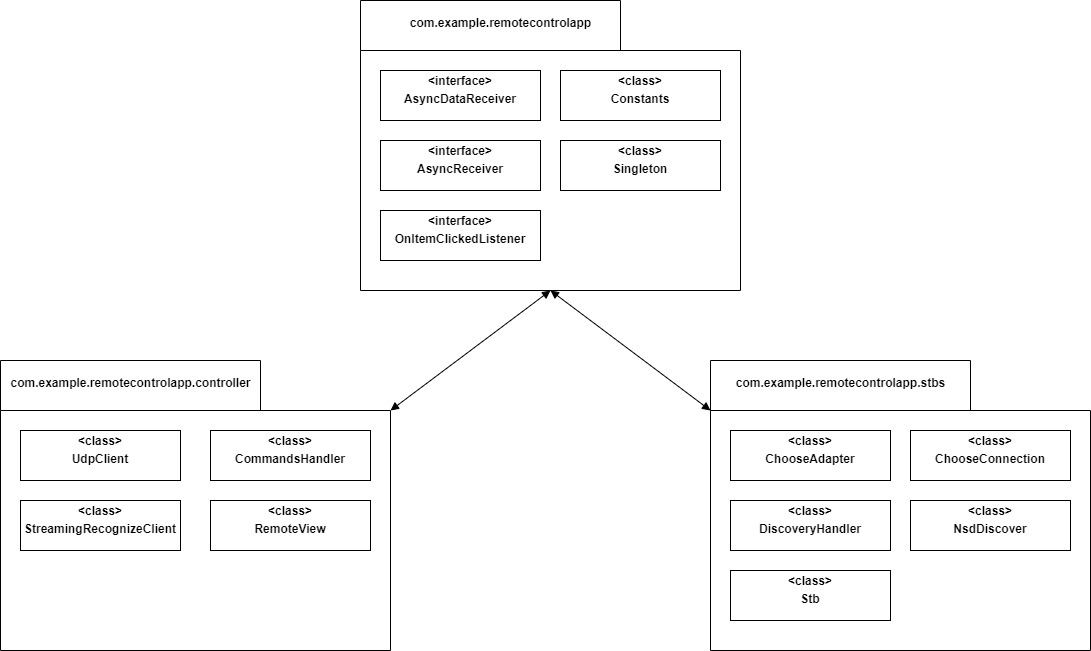
\includegraphics[width=\textwidth]{Implementacija/dijagrami/pakage_diagram.jpg}
  \caption{Dijagram paketa}
  \label{fig:dijagramPaketa}
\end{figure}
%=====================================================================

Klase unutar paketa \textbf{stbs} su:
\begin{itemize}
\item \textit{ChooseAdapter} koja se koristi za prikaz liste pronađenih uređaja,
\item \textit{ChooseConnection} koja se koristi za odabir i povezivanje sa izabranim uređajem,
\item \textit{DiscoveryHandler} koja se koristi za pronalaženje dostupnih uređaja na mreži,
\item \textit{NsdDiscover} koja se koristi za korišćenje NSD (eng. \textit{Network Service Discovery}) mehanizma za pronalaženje uređaja i
\item \textit{Stb} koja predstavlja jedan uređaj i sadrži informacije o njemu.
\end{itemize}
Dijagram klasa ovog paketa se može videti na slici \ref{fig:dijagramStbs}.


%=================== SLIKA ======================================
\begin{figure}[!ht]
  \centering
  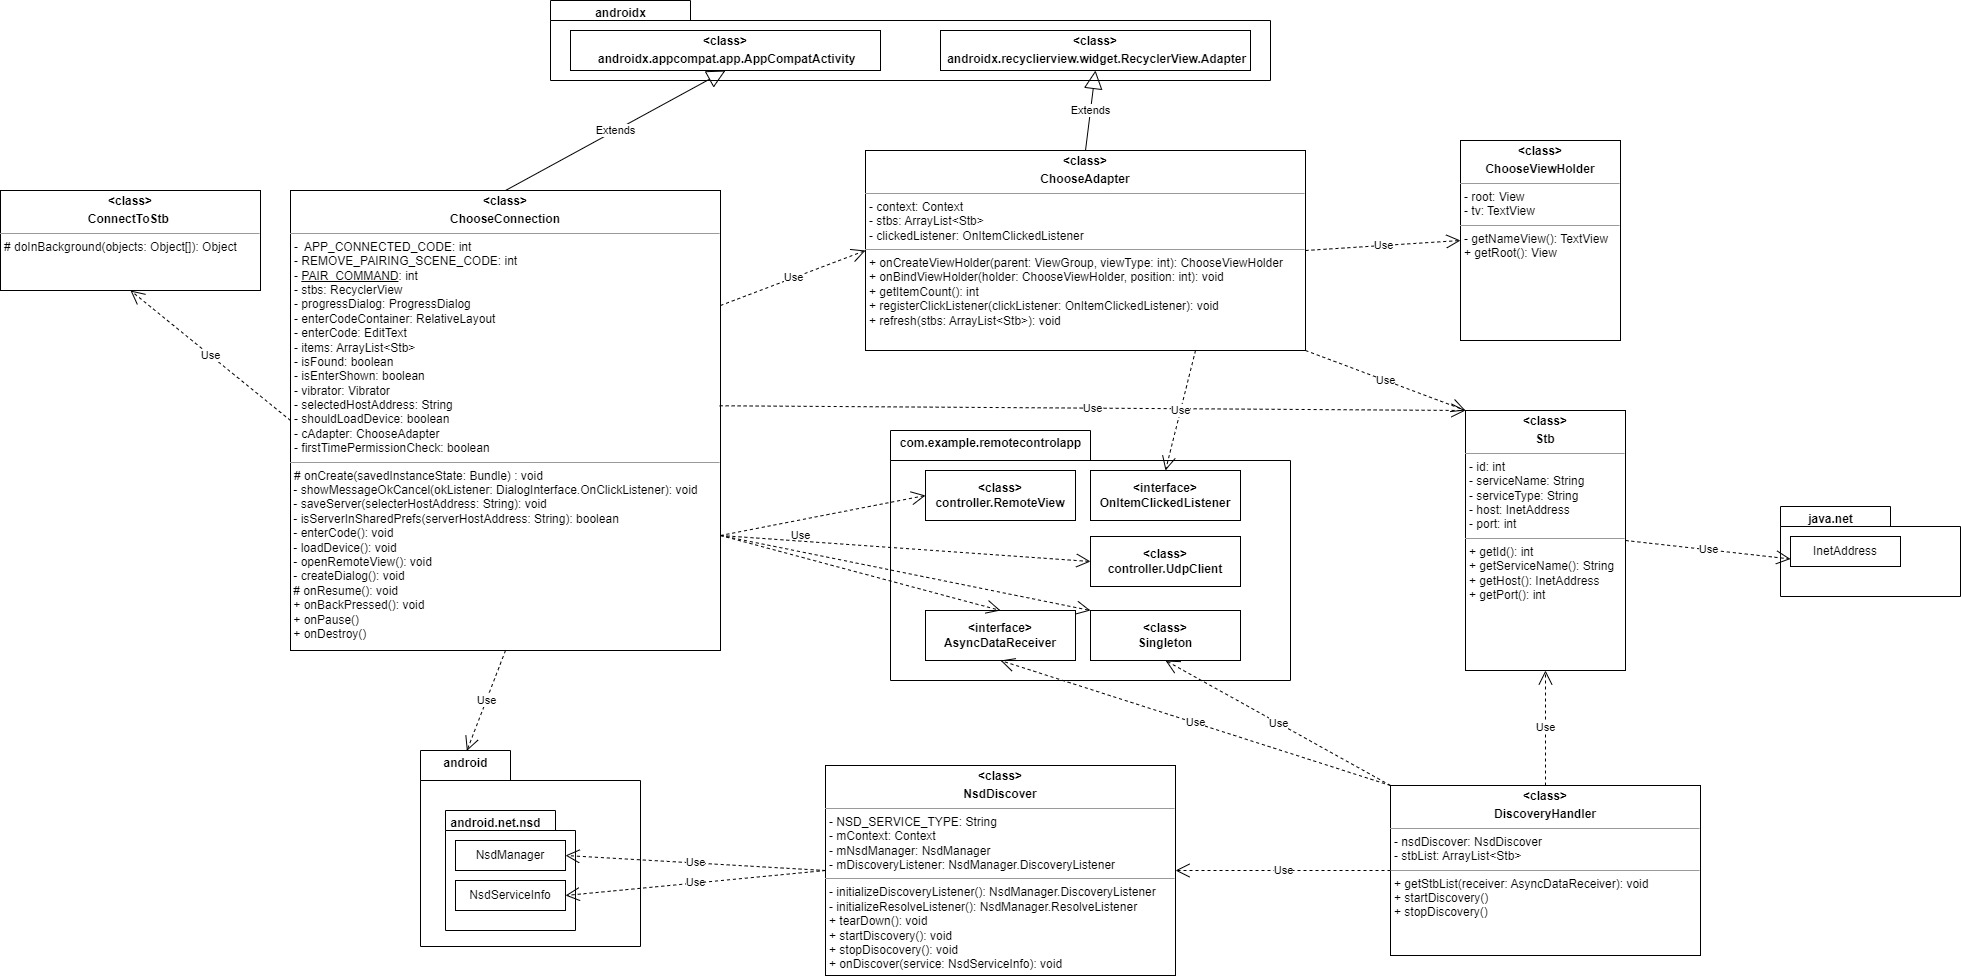
\includegraphics[width=\textwidth]{Implementacija/dijagrami/stbs_pakage_class_diagram.jpg}
  \caption{Dijagram klasa za paket stbs}
  \label{fig:dijagramStbs}
\end{figure}
%=====================================================================

Klase unutar paketa \textbf{controller} su:
\begin{itemize}
\item \textit{CommandsHandler} koja je odgovorna za obradu i slanje komandi na uređaj,
\item \textit{RemoteView} koja se bavi prikazom daljinskog upravljača i interakcijom korisnika sa aplikacijom,
\item \textit{UdpClient} koja omogućava komunikaciju putem UDP protokola i
\item \textit{StreamingRecognizeClient} koje se koristi za obradu audio podataka i prepoznavanje govora pomoću \textit{Google Cloud API}-ja. 
\end{itemize}
Komunikacija i izgled ovih klasa su prikazani na dijagramu \ref{fig:dijagramController}.


%=================== SLIKA ======================================
\begin{figure}[!ht]
  \centering
  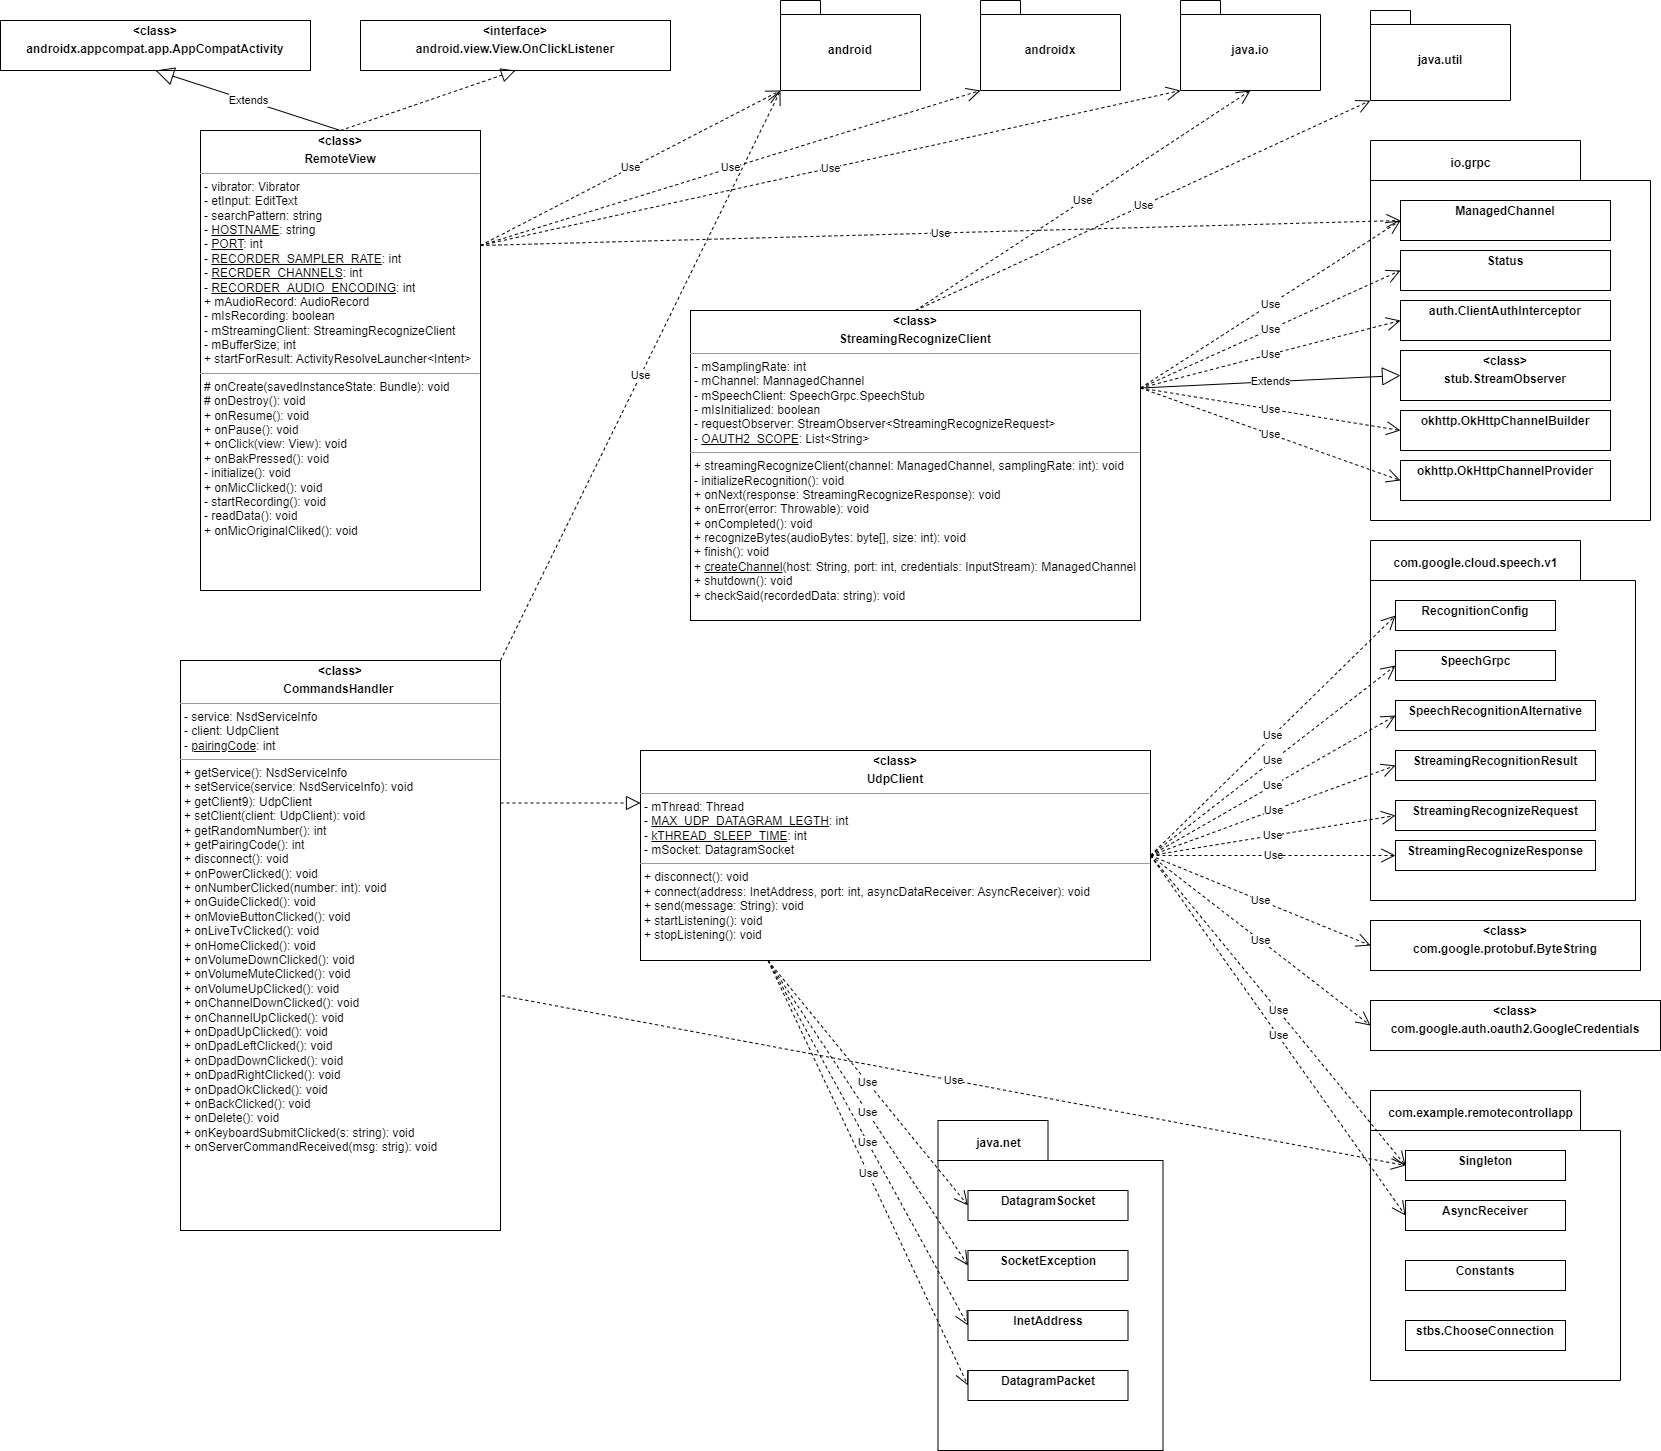
\includegraphics[width=\textwidth]{Implementacija/dijagrami/controller_package_class_diagram.jpg}
  \caption{Dijagram klasa za paket controller}
  \label{fig:dijagramController}
\end{figure}
%=====================================================================

Pored ovih klasa u glavnom paketu aplikacjie nalaze se sledeće klase i interfejsi:
\begin{itemize}
\item Interfejs \textit{AsyncDataReceiver} se koristi kada je potrebno vratiti specifične podatke nakon završetka asinhrone operacije.,
\item Interfejs \textit{AsyncReceiver} se koristi kada je potrebno samo obavestiti o uspehu ili neuspehu asinhrone operacije bez vraćanja specifičnih podataka,
\item Interfejs \textit{OnItemClickedListener} se koristi za obradu klikova na elemente liste,
\item Klasa \textit{Singleton} se koristi za implementaciju Singlton (eng. \textit{Singleton}) šablona,
\item Klasa \textit{Constants} se koristi da skladišti sve konstante potrebne u razvoju aplikacije.
\end{itemize}
Njihov dijagram klasa je prikazan na slici \ref{fig:dijagramRoot}.

%=================== SLIKA ======================================
\begin{figure}[!ht]
  \centering
  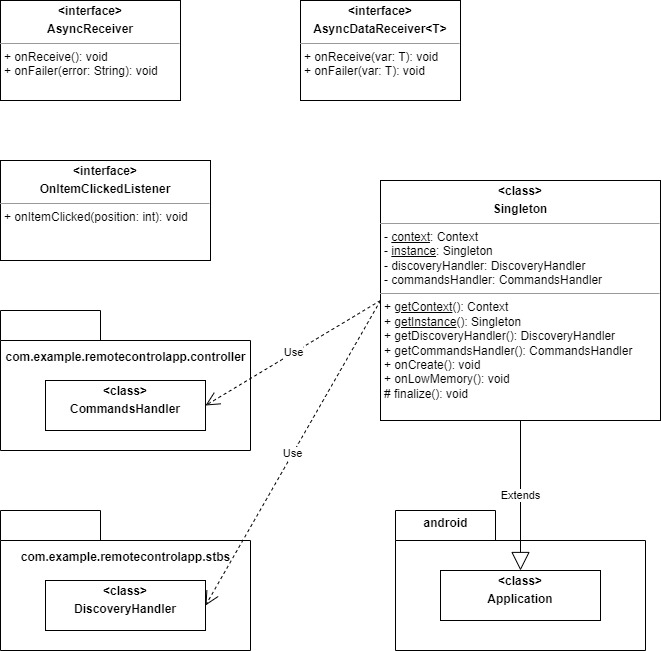
\includegraphics[width=\textwidth]{Implementacija/dijagrami/app_root_package.jpg}
  \caption{Dijagram klasa za glavni paket aplikacije}
  \label{fig:dijagramRoot}
\end{figure}
%=====================================================================

\section{Implementacija glavnih funkcionalnosti aplikacije}
Kao što je navedeno u delu \ref{opis_rada} postoje koraci koji su potrebni da se ispune kako bi se aplikacija koristila za upravljanje uređajem za digitalnu televiziju. U nastavku će biti prikazani delovi koda i objašnjenja kako implementirati pretragu uređaja na mreži, povezivanje sa odabranim uređajem kao i komunikaciju i slanje komandi na uređaj. Poseban osvrt će biti na implementaciji zadavanja glasovnih komandi. 

\subsection{Implementacija pretrage uređaja}
\subfile{implementacije/impl_pretraga}


\subsection{Implementacija povezivanja sa odabranim uređajem}
\subfile{implementacije/impl_povezivanje}

\subsection{Implementacija komunikacije sa uređajem i zadavanja komandi}
\subfile{implementacije/impl_komunikacija}


%\subsection{Implementacija zadavanja glasovnih komandi}
\subfile{implementacije/impl_glas}




% slika podele koda src -> Manifets, res, com, proto + gradle
% Manifest sta ima, glavni delovi
% gradle kako je podesen
% res folder, ukratko xml implementacije neki specif. stvari
% com folder -> tu imamo 2 paketa + ovi glavni
% proto kad i zasto je koriscen
\end{document}